\documentclass[10pt]{examdesign}
\usepackage{amsmath}
\usepackage{enumitem}
\usepackage{amsfonts}
\usepackage{pgfplots}
\usepackage{pifont}
\usepackage{graphicx}
\usepackage{fancyhdr}
\usepackage{cancel}
\usepackage{graphicx}

\SectionFont{\large\sffamily}
\Fullpages
\ContinuousNumbering
\usepackage{ulem}
\ProportionalBlanks{2}


\DefineAnswerWrapper{}{}
\NumberOfVersions{3}
%\IncludeFromFile{foobar.tex}
\examname{Semester 2 REVIEW}
\class{ {\Large Physics}}

\def \namedata {Name: \hrulefill\\ 
	Date: \hrulefill \\
	Period: \hrulefill
	
}




\begin{document}




\begin{multiplechoice} [title={Multiple Choice (3 Points Each)},
	rearrange=No]
	\textit{Choose the best answer to each question.} 
	
	\begin{question}
	A lens has a focal length of -5 cm.  Which statements must be true?
		\choice{The image must be real.}
		\choice{The image must be virtual}
		\choice{The image must be upright.}
		\choice{The image must be inverted.}
		\choice[!]{The image must be smaller.}
		\choice{The image must be larger.}
	\end{question}



	\begin{question}
	A penny is placed in the bottom of a cup, and the cup is placed so that the penny is just outside the person's view, as shown in the picture.  If the cup is carefully filled with water without causing the penny to move, what will happen?
		
	\begin{center} 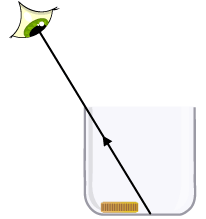
\includegraphics[width=1.25in]{penny.png} \end{center}

\end{question}

\begin{block}
	
	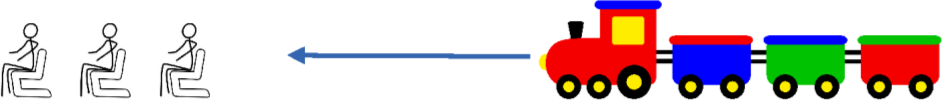
\includegraphics[width=5in]{train.png} 
	
	
	\begin{question}
		A train is moving at 25 m/s as it is approaching a train station where several students are sitting in chairs, as shown above.  If the train's whistle has a frequency of 700 Hz, the frequency the people hear is - 

	\end{question}
\end{block}


\begin{question}
	The number of times that a wave repeats itself in one second is known as its - 

	
	\end{question}

	\begin{question}
	Kinetic Energy is best defined as - 

	\end{question}
	
	\begin{question}
	The energy stored in a spring when it is stretched is called - 
	\end{question}
	
	\begin{question}
	A planet is found that is the exact same mass as Earth, and has all the conditions needed to support life, (oxygen, water, sunlight, etc) but there is no life on the planet.  An astronaut plants some grass and drops off some cows and bull.  Over the next thousand years, the grass grows and the cows reproduce.  If no other trips are made to visit the planet, the total mass of this planet (including the mass of the cows and the grass)
		\choice{Increases as the grass grows and the cows reproduce.}
		\choice[!]{Remains constant due to the law of conservation of mass.}
		\choice{Decreases due to the cows eating the grass.}
		\choice{Could increase, decrease, or remain the same depending on the final number of cows and total amount of grass after 1000 years.}
	\end{question}

	\begin{question}
	A pendulum of length $ \ell $ has a period of 1 second.  What would the period of a pendulum of length $ 5\ell $ be?

	
	\end{question}


	\begin{question}
	A 3 kg block hangs from a spring that is attached to the ceiling of an elevator.  As the elevator accelerates upward, the spring - 
	\choice[!]{Gets longer}
	\choice{Gets shorter}
	\choice{Remains the same length}
	\choice{It cannot be determined without knowing the spring constant and the acceleration of the elevator.}
	\end{question}




	\begin{question}
	A wheel spins thirteen times.  What is the angle (in radians) that the wheel has traveled?

	\end{question}

\begin{block}
	
	\textbf{The following two questions refer to the following information:} 
	The picture below shows an overhead view of China's Z-20 Anti-submarine helicopter.  Two points have been labeled A and B.  
	
	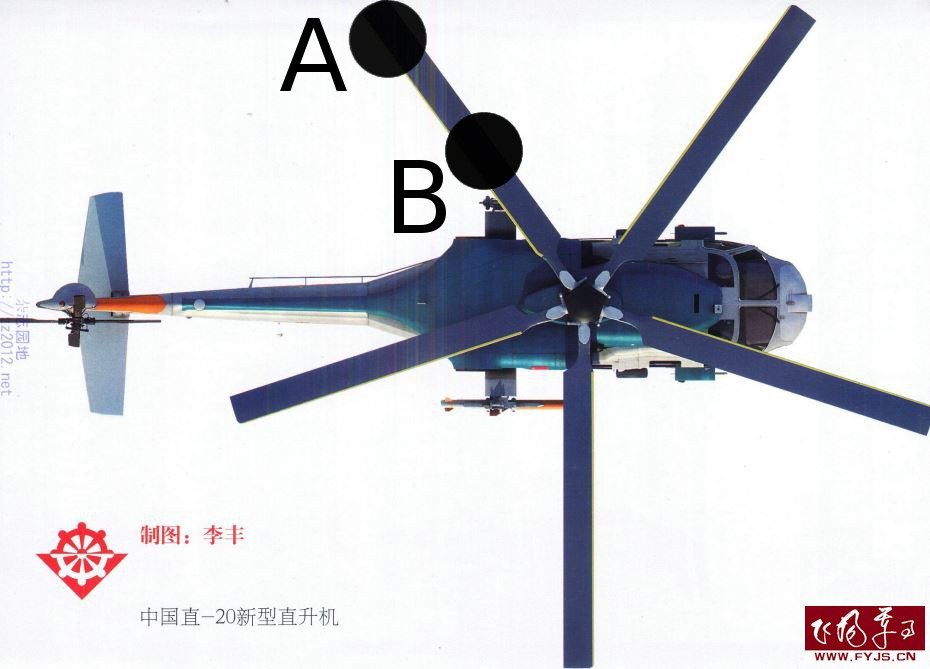
\includegraphics[height=3cm]{heli.jpg}
	
	
	
	\begin{question}
		When the helicopter blades are rotating, which point has a greater \underline{angular velocity ($\omega$)}?
		
		\vspace{0.1in}
		
		\choice{A}
		\choice{B}
		\choice[!]{They both have the same angular velocity}
		\choice{It is impossible to tell.}
	\end{question}
	
	\begin{question}
		When the helicopter blades are rotating, which point has a greater \underline{linear velocity (v)}?
		
		\vspace{0.1in}
		
		\choice{A}
		\choice{B}
		\choice[!]{They both have the same angular velocity}
		\choice{It is impossible to tell.}
	\end{question}
	
	
	
\end{block}

\begin{block}
	
	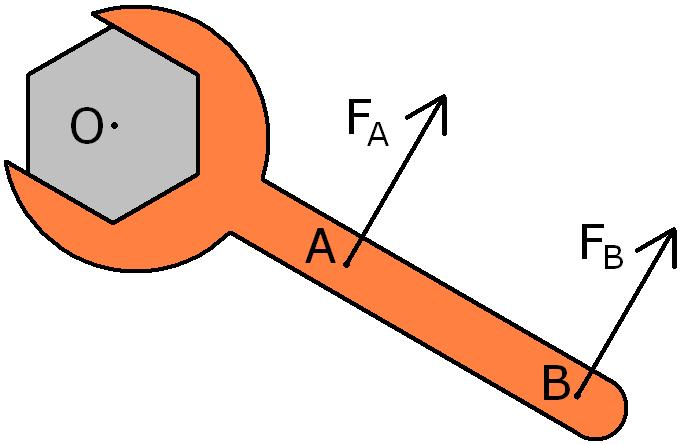
\includegraphics[height=3cm]{wrench.png}

	
\begin{question}

You are attempting to loosen a bolt from your car by putting a force on a wrench, as shown in the picture.   You can choose to put a force on the wrench at point A or at point B.  If both the forces are the same magnitude, which force is more effective in loosening the bolt?

\end{question}
\end{block}

\begin{question}
Bats use ultrasonic sounds of 25000 Hz to find bugs by echolocation.  A bat is flying 7 m/s to the right.  A bug is to the right of the bat, and hears a sound of 26500 Hz.  Describe the motion of the bat.
\end{question}

\begin{question}
	While you are driving on the highway, a bug collides with the windshield of your car.  The impulse on the bug is - 
	\choice [!]{equal to the impulse on the car and in the opposite direction.}
	\choice {less than the impulse on the car and in the same direction.}
	\choice {greater than the impulse on the car and in the opposite direction.}
	\choice {equal to the impulse on the car and in the same direction. }
\end{question}


\begin{question}
	An object is placed 6 cm to the left of a lens.  A real image forms 4 cm to the right of the lens.  What is the focal length of the lens?
	
\end{question}

\begin{question}
 Corn Syrup has an index of refraction of 1.60.  What is the speed of light in corn syrup?

\end{question}

\begin{question}
	In marching band, Emily plays an \textit{A} on her clarinet (f = 440 Hz) as she marches forward at 4 m/s.  What frequency would a spectator in the stands hear? 

\end{question}

\begin{question}
	An ocean wave moves toward the shore at 3m/s.  It has a period of 5 seconds.  What is its wavelength?

\end{question}



\begin{question}
	What is the kinetic energy of a 2000 kg car that travels at 20 m/s?

\end{question}

\begin{question}
	An Eagle drops a clam from a height of 23 m in order to break its shell open.  What is the speed of the clam as it hits the ground?

	
\end{question}

	\begin{question}
	A hunting whale is swimming at 7 m/s when it catches a sleeping giant squid of the same mass in its mouth.  Immediately after catching the squid, how fast will the two be moving?

\end{question}



\begin{question}
	A pendulum has a length of 0.5m.  What is its period?

\end{question}


\begin{question}
	A spring has 0.5 J of elastic potential energy when it is stretched 0.03m.  What is the spring constant of the spring?

\end{question}


\begin{block}
		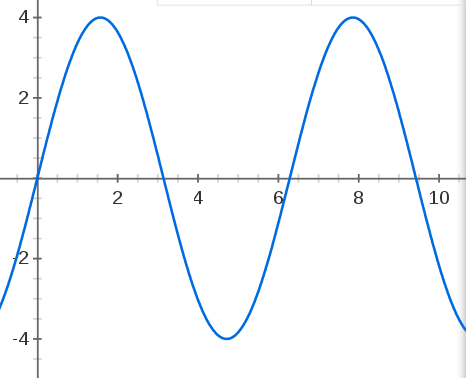
\includegraphics[height=4cm]{wave2.png}
	
\begin{question}
	What is the approximate amplitude of the wave shown above?

	\end{question}

\end{block}


\begin{question}
A regulation basketball (m=0.625 kg) and a 12-pound bowling ball (m=5.44311 kg) are allowed to roll down a ramp.  The moment of inertia of a solid sphere is $I = \frac{2}{5} mr^2$, and the moment of inertia for a hollow sphere is $I = \frac{2}{3} mr^2$.  Which object reaches the bottom of the ramp first?

\end{question}



\begin{question}
	A dog is at the back of an empty boat when he sees an interesting fish jump near the front of the boat.  The dog runs 3 meters east, to the front of the boat, then stops.  The dog has a mass of 30kg, and the boat has a mass of 60 kg.  If there is no friction between the boat and the water, how far does the boat move? 

\end{question}


	\begin{question}
	Which of the following is the best example of an \textbf{\underline{inelastic}} collision.
	\choice{William dribbles a basketball.}
	\choice{Diego kicks a soccer ball.}
	\choice[!]{Victor throws his gum and it sticks to the wall.}
	\choice{Martin punches the wall and makes a hole in it.}
\end{question}

\end{multiplechoice}

\end{document}
